\documentclass[11pt]{article}

%%%%%%%%%%%%
% Packages %
%%%%%%%%%%%%

\hyphenpenalty=10000
\usepackage{tikz}
\usetikzlibrary{shapes,arrows}

\usepackage{tocloft}
\renewcommand\cftsecleader{\cftdotfill{\cftdotsep}}
\def\undertilde#1{\mathord{\vtop{\ialign{##\crcr
$\hfil\displaystyle{#1}\hfil$\crcr\noalign{\kern1.5pt\nointerlineskip}
$\hfil\tilde{}\hfil$\crcr\noalign{\kern1.5pt}}}}}
\usepackage{cleveref}
\usepackage{xcolor}
\usepackage[colorlinks = true,
            linkcolor = black,
            urlcolor  = black,
            citecolor = black,
            anchorcolor = black]{hyperref}
\usepackage{epstopdf}
\usepackage{braket}
\usepackage{upgreek}
\usepackage{caption}
\usepackage{booktabs}
\usepackage{subcaption}
\usepackage{amssymb,latexsym,amsmath,gensymb}
\usepackage{latexsym}
\usepackage{graphicx}
\usepackage{float}
\usepackage{enumitem}
\usepackage{pdflscape}
\usepackage{url}
\usepackage{array}
\newcolumntype{C}{>{$\displaystyle} c <{$}}
\usepackage{tikz, calc}
\usetikzlibrary{shapes.geometric, arrows, calc}
\tikzstyle{norm} = [rectangle, rounded corners, minimum width=2cm, minimum height=1cm,text centered, draw=black]
\tikzstyle{arrow} = [thick, ->, >=stealth]

\newcommand{\argmin}{\arg\!\min}
\newcommand{\me}{\mathrm{e}}
\providecommand{\e}[1]{\ensuremath{\times 10^{#1}}} 
\providecommand{\mb}[1]{\mathbf{#1}}
\providecommand{\mf}[1]{\mathbf{#1}}
\providecommand{\ro}[1]{\mathbf{\mathbf{r}}_o}
\providecommand{\so}[1]{\mathbf{\hat{s}}_o}
\providecommand{\rb}[1]{\mathbf{r}_b}
\providecommand{\rbm}[1]{r_b^{\text{m}}}
\providecommand{\rd}[1]{\mathbf{r}_d}
\providecommand{\mh}[1]{\mathbf{\hat{#1}}}
\providecommand{\bs}[1]{\boldsymbol{#1}} 
\providecommand{\intinf}{\int_{-\infty}^{\infty}}
\providecommand{\fig}[4]{
  % filename, width, caption, label
\begin{figure}[h]
 \captionsetup{width=1.0\linewidth}
 \centering
 \includegraphics[width = #2\textwidth]{#1}
 \caption{#3}
 \label{fig:#4}
\end{figure}
}

\newcommand{\tensor}[1]{\overset{\text{\tiny$\leftrightarrow$}}{\mb{#1}}}
\newcommand{\tunderbrace}[2]{\underbrace{#1}_{\textstyle#2}}
\providecommand{\figs}[7]{
  % filename1, filename2, caption1, caption2, label1, label2, shift
\begin{figure}[H]
\centering
\begin{minipage}[b]{.45\textwidth}
  \centering
  \includegraphics[width=1.0\linewidth]{#1}
  \captionsetup{justification=justified, singlelinecheck=true}
  \caption{#3}
  \label{fig:#5}
\end{minipage}
\hspace{2em}
\begin{minipage}[b]{.45\textwidth}
  \centering
  \includegraphics[width=1.0\linewidth]{#2}
  \vspace{#7em}
  \captionsetup{justification=justified}
  \caption{#4}
  \label{fig:#6}
\end{minipage}
\end{figure}
}
\makeatletter

\providecommand{\code}[1]{
\begin{center}
\lstinputlisting{#1}
\end{center}
}

\newcommand{\crefrangeconjunction}{--}
%%%%%%%%%%%
% Spacing %
%%%%%%%%%%%
% Margins
\usepackage[
top    = 1.5cm,
bottom = 1.5cm,
left   = 1.5cm,
right  = 1.5cm]{geometry}

% Indents, paragraph space
%\usepackage{parskip}
\setlength{\parskip}{1.5ex}

% Section spacing
\usepackage{titlesec}
\titlespacing*{\title}
{0pt}{0ex}{0ex}
\titlespacing*{\section}
{0pt}{0ex}{0ex}
\titlespacing*{\subsection}
{0pt}{0ex}{0ex}
\titlespacing*{\subsubsection}
{0pt}{0ex}{0ex}

% Line spacing
\linespread{1.1}

%%%%%%%%%%%%
% Document %
%%%%%%%%%%%%
\begin{document}
\title{\vspace{-2.5em} Spatio-angular transfer functions for fluorescence microscopes\vspace{-1em}}  \author{Talon Chandler, Min Guo, Hari Shroff, Rudolf Oldenbourg, Patrick La Rivi\`ere}
\date{\vspace{-1em}\today\vspace{-1em}}
\maketitle
\begin{abstract}
  We investigate how the orientation and position of fluorescent dipole emitters
  affects microscopic imaging using electromagnetic optics theory. Starting with
  the thoroughly studied spatio-angular point spread function, we introduce the
  spatio-angular coherent spread function, coherent transfer function, and
  optical transfer function as electromagnetic extensions of well-known
  functions in scalar optics theory. We use these concepts to show that
  fluorescence microscopes have a spatio-angular band limit. Finally, we study
  polarized light microscopes and find that polarized illumination is a type of
  structured illumination that extends the angular band limit.
\end{abstract}
\section{Introduction}
TODO

We use plain roman type for scalars, e.g., $x, y, z$; bold lowercase roman type
for two-dimensional vectors, e.g., $\mb{r}$; hats for unit vectors, e.g.,
$\mb{\hat{s}}$; and bold capital roman type for matrices, e.g.,
$\mb{R}$. We use the real spherical harmonic functions
\begin{align}
  y_l^m(\vartheta, \varphi) =
  \begin{cases}
    \sqrt{2}K_l^m\cos(m\varphi)P_l^m(\cos\vartheta), & m > 0\\
    K_l^0P_l^0(\cos\vartheta), & m = 0\\
    \sqrt{2}K_l^m\sin(-m\varphi)P_l^{-m}(\cos\vartheta), & m < 0\\
  \end{cases}
\end{align}
where
\begin{align}
  K_l^m = \sqrt{\frac{(2l+1)}{4\pi}\frac{(l-|m|)!}{(l+|m|)!}},
\end{align}
and $P_l^m(x)$ are the associated Legendre polynomials. The $l=0$ and $l=1$
spherical harmonics are given by
\begin{equation}
\begin{aligned}
  y_0^0(\vartheta, \varphi) &= \sqrt{\frac{1}{4\pi}},\\
  y_1^{-1}(\vartheta, \varphi) = \sqrt{\frac{3}{4\pi}}\sin\varphi\sin\vartheta, \hspace{2em} y_1^0(\vartheta, \varphi) &= \sqrt{\frac{3}{4\pi}}\cos\vartheta, \hspace{2em} y_1^1(\vartheta, \varphi) = \sqrt{\frac{3}{4\pi}}\cos\varphi\sin\vartheta. \label{eq:harmonics}
\end{aligned}
\end{equation}

\section{Spatio-angular point spread functions}
\begin{figure}[h]
 \captionsetup{width=1.0\linewidth}
 \centering
   \centering
   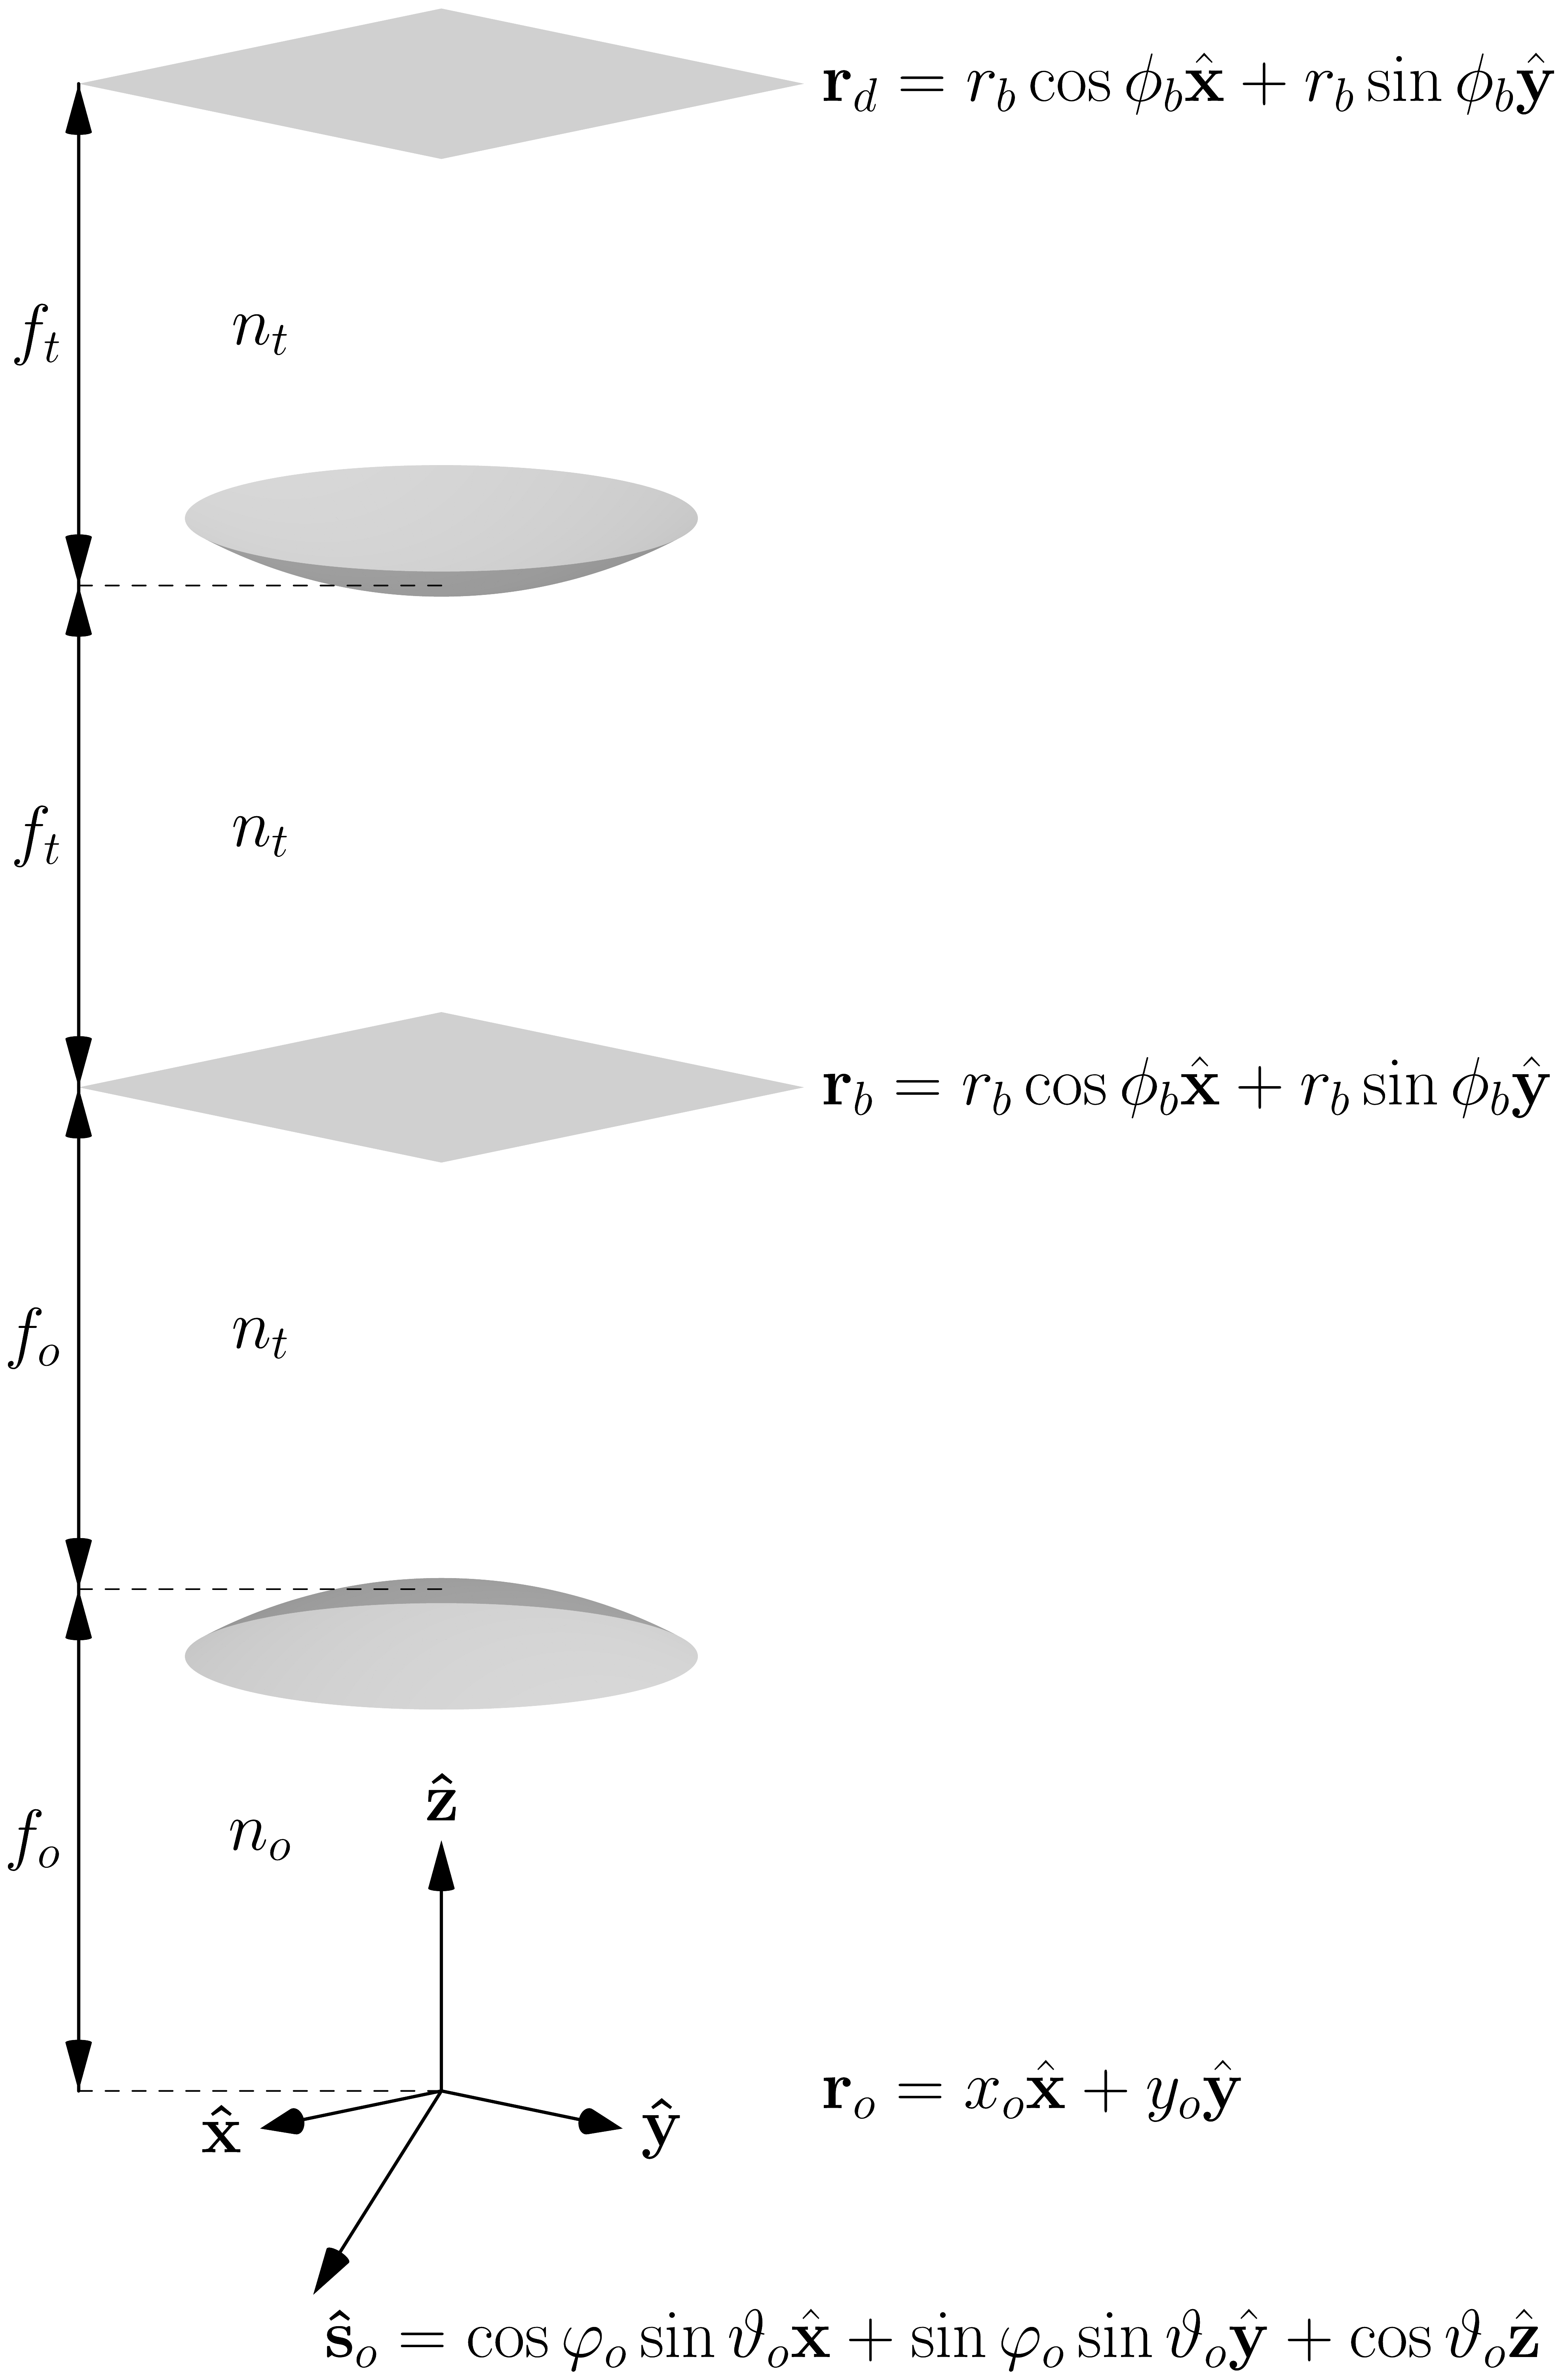
\includegraphics[width = 0.4\textwidth]{../figures/schematic.pdf}
   \caption{Simplified schematic of a single-view fluorescence microscope. The
     object is placed near the focal point of an aplanatic objective lens with
     focal length $f_{o}$ in a medium with refractive index $n_o$. The object is
     parameterized by the 2D position vector $\ro{}$ ($o$ for object) and an
     orientation unit vector $\so{}$. The light emitted by the fluorescent
     object is collected and collimated by the objective lens so that the
     electric fields are purely transverse in the back focal plane. Points in
     the back focal plane are parameterized by a 2D position vector $\rb{}$ ($b$
     for back focal plane). Finally, the tube lens with focal length $f_t$
     refocuses the light onto a detector. Points on the detector are
     parameterized by a 2D position vector $\rd{}$ ($d$ for detector). The back
     focal plane and detector are in a medium with refractive index $n_t$. Note
     that this schematic is not to scale---we consider the case where
     $f_o \ll f_t$.}
   \label{fig:frames_a}
\end{figure}

Figure \ref{fig:frames_a} shows a schematic of the fluorescence microscope that
we are considering with a summary of our notation. We start by following Backer
and Moerner \cite{backer2014} to find the electric field at position $\rb{}$ in
the back focal plane due to a single dipole emitter at position $\ro{}$ oriented
along $\so{}$ as
\begin{align}
  \mb{\tilde{e}}_b(\rb{};\ro{}, \so{}) \propto \me^{-i(kn_o/f_o)\rb{}\cdot\ro{}}\sqrt{\frac{1}{\rho_b}}
  \begin{bmatrix}
    \sin^2\phi_b + \rho_b\cos^2\phi_b&\sin\phi_b\cos\phi_b(\rho_b - 1)&-\frac{r_b}{f_o}\cos\phi_b\\
    \sin\phi_b\cos\phi_b(\rho_b - 1)&\cos^2\phi_b + \rho_b\sin^2\phi_b&-\frac{r_b}{f_o}\sin\phi_b\\
    0&0&0
  \end{bmatrix}
  \begin{bmatrix}
    \cos\varphi_o\sin\vartheta_o\\
    \sin\varphi_o\sin\vartheta_o\\
    \cos\vartheta_o
  \end{bmatrix}
\Pi\left(\frac{r_b}{r_b^{\text{max}}}\right)\label{eq:bfp}
\end{align}
where we define $\rho_b \equiv \sqrt{1 - \left(\frac{r_b}{f_o}\right)^2}$, and
$\Pi(x)$ is a boxcar function that returns 1 when $|x| < 1$ and 0 otherwise. We
can understand this expression term by term---the exponential term accounts for
the phase as dipole emitter is moved in object space, the square root term
conserves power before and after the objective lens, the matrix models the
dipole emission process and electric field rotation caused by the objective
lens, the vector is the dipole orientation unit vector, and
$\Pi\left(\frac{r_b}{r_b^{\text{max}}}\right)$ accounts for the numerical
aperture of the lens with $r_b^{\text{max}} = \frac{f_0}{n_0}\text{NA}$. We use
a tilde to mark single dipole response functions---we will consider the response
due to a field of dipoles in the next section.

If the tube lens is weakly focusing ($f_o \ll f_t$) then we can find the
electric field in the detector plane by taking the Fourier transform of the
electric field in the back focal plane
\begin{align}
  \mb{\tilde{e}}_d(\rd{}; \ro{}, \so{}) \propto \int_{\mathbb{R}^2} d\rb{}\, \tilde{\mb{e}}_b(\rb{}; \ro{}, \so{})\me^{-i (kn_t/f_t) \rb{} \cdot \rd{}}. \label{eq:ed}
\end{align}
By isolating the phase term in Eq. \ref{eq:bfp} with
$\mb{\tilde{e}}_b(\rb{};\ro{}, \so{}) = \me^{-i(kn_o/f_o)\rb{}\cdot\ro{}}
\tilde{\underline{\mb{e}}}_b(\rb{};\ro{}, \so{})$, and plugging into Eq. \ref{eq:ed} we find
that 
\begin{align}
  \mb{\tilde{e}}_d(\rd{} - M\ro{}, \so{}) \propto \int_{\mathbb{R}^2} d\rb{}\, \tilde{\underline{\mb{e}}}_b(\rb{}; \ro{}, \so{})\me^{-i (kn_t/f_t)\, \rb{} \cdot [\,\rd{} - M\ro{}]}.
\end{align}
where $M = -\frac{n_o}{n_t}\frac{f_t}{f_o}$ is the transverse magnification.  By
writing the electric field in the detector plane in terms of $\rd{} - M\ro{}$,
we have established that the electric field in the detector plane is
\textit{transverse shift-invariant}---a transverse shift of the object creates a
magnified transverse shift of the image. We define coordinates on the detector
centered on the image of the object
$\rd{}' \equiv \rd{} - M\ro{} = r_d'\cos\phi_d'\mh{x} + r_d'\sin\phi_d\mh{y}$,
then we follow Novotny \cite{nov2006} by writing the integrals in polar
coordinates, evaluating the azimuthal integrals, and writing the result
concisely in terms of three radial integrals
\begin{align}
  \tilde{\mb{e}}_d(\rd{}', \so{}) &\propto
  \begin{bmatrix}
    A + C\cos(2\phi_d') & C\sin(2\phi_d') & -2iB\cos\phi_d'\\
    C\sin(2\phi_d') & A - C\cos(2\phi_d') & -2iB\sin\phi_d'\\
    0&0&0\\
  \end{bmatrix}
  \begin{bmatrix}
    \cos\varphi_o\sin\vartheta_o\\
    \sin\varphi_o\sin\vartheta_o\\
    \cos\vartheta_o
  \end{bmatrix}\label{eq:elec}
\end{align}
where $A, B$ and $C$ are
\begin{align}
  A(r_d') &= \int_0^{\theta_{\text{max}}}d\theta\ \sqrt{\cos\theta}\sin\theta(1+\cos\theta)J_0(k_b r_d'\sin\theta f_o/f_t),\\%\ \text{exp}\left\{ik_bz_o[1-(1/2)(f_o/f_t)^2\sin^2\theta]\right\},\\
  B(r_d') &= \int_0^{\theta_{\text{max}}}d\theta\ \sqrt{\cos\theta}\sin^2\theta J_1(k_b r_d'\sin\theta f_o/f_t),\\%\ \text{exp}\left\{ik_bz_o[1-(1/2)(f_o/f_t)^2\sin^2\theta]\right\},\\
  C(r_d') &= \int_0^{\theta_{\text{max}}}d\theta\ \sqrt{\cos\theta}\sin\theta(1-\cos\theta)J_2(k_b r_d'\sin\theta f_o/f_t).%\ \text{exp}\left\{ik_bz_o[1-(1/2)(f_o/f_t)^2\sin^2\theta]\right\}.
\end{align}
We can identify Eq. \ref{eq:elec} as the vector-valued \textit{coherent spread
  function} (CSF) of the microscope. The scalar-valued CSF---sometimes called
the amplitude transfer function---is only applicable to cases where
electromagnetic optics plays no role in the microscope---not true
for oriented samples. 

To build our intuition about the CSF, we will rewrite the matrix multiplication
in Eq. \ref{eq:elec} in terms of the spherical harmonics. Notice that the $l=1$
spherical harmonics are the Cartesian components of the unit dipole axis (see
Eq. \ref{eq:harmonics}), so the CSF becomes
\begin{align}
  \tilde{\mb{e}}_d(\rd{}', \so{}) &\propto
  \begin{bmatrix}
    [A + C\cos(2\phi_d')]y_1^{1}(\so{}) + C\sin(2\phi_d')y_1^{-1}(\so{}) - 2iB\cos\phi_d'y_1^{0}(\so{})\\
    C\sin(2\phi_d')y_1^{1}(\so{}) + [A - C\cos(2\phi_d')]y_1^{-1}(\so{}) - 2iB\sin\phi_d'y_1^{0}(\so{})\\
    0\\
  \end{bmatrix}.
\end{align}
By applying the paraxial approximation ($\sin\theta\approx\theta$ and
$\cos\theta\approx 1$), the integrals $A, B$ and $C$ can be evaluated in terms
of Bessel functions. We can evaluate $A$ and $B$ with the help of
$\int_0^zdx\ xJ_0(ax) = zJ_1(az)/a$ and $\int_0^zdx\ x^2J_1(ax) = z^2J_2(az)/a$,
respectively, and $C = 0$ because $J_2(x)$ is zero to first order. In this
case, the CSF simplifies to
\begin{align}
  \tilde{\mb{e}}^{(p)}_d(\rd{}', \so{}) &\propto
  \begin{bmatrix}
    A^{(p)}y_1^{1}(\so{}) - 2iB^{(p)}\cos\phi_d'y_1^{0}(\so{})\\
    A^{(p)}y_1^{-1}(\so{}) - 2iB^{(p)}\sin\phi_d'y_1^{0}(\so{})\\
    0\\
  \end{bmatrix}\label{eq:paracsf}
\end{align}
where the integrals evaluate to
\begin{align}
  {A^{(p)}} = \frac{2J_1(\tilde{r}_d)}{\tilde{r}_d},
  \hspace{2em}
    {B^{(p)}} = \frac{\text{NA}}{n_o}\left[\frac{2J_2(\tilde{r}_d)}{\tilde{r}_d}\right],
  \intertext{and we have substituted}
  \tilde{r}_d = \frac{2\pi\text{NA}\thinspace r_d}{M\lambda},\hspace{2em}
  \text{NA} = n_o\sin\theta_{\text{max}}.
\end{align}
We will continue to use an superscipt $(p)$ to mark the terms where we have used
the paraxial approximation.

Under the paraxial approximation the electric fields on the detector created by
a single dipole are composed of two parts, a parallel part and a radial
part. The coefficients of the $y_1^0$ spherical harmonic in Eq. \ref{eq:paracsf}
create the radial part of the field---the $z$ component of the dipole generates
a radial field on the detector with respect to the image point. The coefficients
of the $y_1^1$ and $y_1^{-1}$ spherical harmonics create a parallel field in the
detector plane parallel to the $x$ and $y$ components of the
dipole. As the NA increases and the paraxial approximation no longer applies, we
begin to see coupling between the $x(y)$ component of the dipole with the $y(x)$
transverse field.

We can find the intensity in the detector plane due to a single dipole
by taking the modulus squared of the CSF
\begin{align}
  \tilde{h}(\rd{}', \so{}) = \left|\tilde{\mb{e}}_d(\rd{}', \so{})\right|^2 \label{eq:kernel}.
\end{align}
For convenience we keep the CSF written in terms of the spherical harmonics and
use a table of spherical harmonic products (see Appendix \ref{realspherical}) to
calculate the intensity in the detector plane as
\begin{equation}
  \begin{split}
  \tilde{h}(\rd{}', \so{}) \propto &\left(A^2 + 2B^2 + C^2\right)y_0^0(\so{}) -\frac{2\sqrt{15}}{5}AC\sin(2\phi_d')y_2^{-2}(\so{})\\ &+ \frac{1}{\sqrt{5}}\left(-A^2 + 4B^2 - C^2\right)y_2^{0}(\so{}) +\frac{2\sqrt{15}}{5}AC\cos(2\phi_d')y_2^{2}(\so{}). \label{eq:kerna}
\end{split}
\end{equation}
We can identify Eq. \ref{eq:kerna} as the spatio-angular \textit{point spread
  function} (PSF) of the microscope. Writing the spatio-angular PSF in terms of
spherical harmonic functions has two advantages. First, it allows us to express
the spatio-angular PSF very concisely. Instead of considering the point spread
function for every possible dipole orientation, we only need to consider four
spatio-angular PSFs---one for each spherical harmonic. Second, the spherical
harmonic functions form an orthonormal basis for functions on the sphere---a
convenient fact that we will use later.

It is useful to compare equation \ref{eq:kerna} to Backer and Moerner's approach
\cite{backer2014}. They expand the spatio-angular PSF in terms of six second
moments of the fluorophore distribution
$\{s_x^2, s_y^2, s_z^2, s_xs_y, s_xs_z, s_ys_z\}$. This approach is very
useful---only six precomputed spatio-angular PSFs are required to represent an
arbitrary spatio-angular PSF. Instead of expanding in terms of six second
moments, we expand onto just four spherical harmonics which, unlike the second
moments, are orthonormal functions. In the next section we will use the
orthonormality of the spherical harmonics to derive spatio-angular transfer
functions for fluorescence microscopes.

The spatio-angular PSF under the paraxial approximation is given by
\begin{align}
      \tilde{h}^{(p)}(\rd{}', \so{}) \propto \left({A^{(p)}}^2 + 2{B^{(p)}}^2\right)y_0^0(\so{}) + \frac{1}{\sqrt{5}}\left(-{A^{(p)}}^2 + 4{B^{(p)}}^2\right)y_2^{0}(\so{})\label{eq:para}.
\end{align}
First, consider the coefficient on the $y_0^0$ spherical harmonic in
Eq. \ref{eq:para}. This coefficient is the point spread function for a angularly
uniform distribution of fluorophores. The first term of the coefficient ${A^{(p)}}^2$
is the familiar Airy disk that arises from the contribution of dipoles oriented
in the transverse plane, while the second term ${B^{(p)}}^2$ is a smaller factor that
arises from dipoles oriented outside of the transverse plane. This leads to an
interesting conclusion---a uniform distribution of dipoles has a point spread
function that is slightly wider than an Airy disk even in the paraxial
approximation. The Airy disk is usually derived using paraxial scalar optics
while here we have used paraxial electromagnetic optics. Therefore, we can
consider the second term to be an electromagnetic correction to the Airy
disk. We will quantify this difference in the next section.

Next, consider the coefficient on the $y_2^0$ spherical harmonic in
Eq. \ref{eq:para}. This coefficient is the spatial PSF for a distribution of
fluorophores proportional to $3\cos^2\vartheta_o - 1$. Counterintuitively, this
fluorophore distribution cannot exist because it would require a negative number
of fluorophores along some orientations; but if this distribution could exist,
then this coefficient would be its spatial PSF. Considering negative
distributions of fluorophores in our calculations should not be cause for
concern. The spherical harmonics span the space of functions on the sphere, so
any positive fluorophore distribution can be represented by the spherical
harmonics and we never need to consider negative fluorophores.
    
Finally, consider all of the spherical harmonics that have a zero
coefficient. These spherical harmonics span the angular null space of our
measurement system---fluorophore distributions that lie in the null space do not
affect the measured intensities. Under the paraxial approximation all of the
non-zero coefficients are rotationally symmetric ($m=0$) spherical harmonics
which means that the transverse orientation of the dipoles does not affect the
PSF. In the high NA case this is no longer true---two $m=2$ spherical harmonics
have non-zero coefficients and the transverse orientation of dipoles does affect
the PSF.


\section{Spatio-angular transfer functions}
Consider a thin object that consists of fluorescent dipoles in arbitrary
positions and orientations. We can represent the entire object using a function
$\bs{\mu}(\ro{}, \so{})$ that returns a complex-valued vector for each position
$\ro{}$ and direction $\so{}$. The magnitude of the complex-valued vector is the
magnitude of the dipole moment and the elements of the vector give the orientation
and phase of the radiating dipole moment. Because $\bs{\mu}(\ro{}, \so{})$
includes the relative phases of different points and orientations in the object,
$\bs{\mu}(\ro{}, \so{})$ can represent coupled dipoles that are emitting
partially or completely coherently.

We can find the electric field on the detector created by this object by
multiplying $\bs{\mu}(\ro{}, \so{})$ with the CSF then integrating over all
positions and orientations in the object
\begin{align}
  \mb{e}_d(\rd{}) = \int_{\mathbb{S}^2}d\so{}\int_{\mathbb{R}^2}d\ro{} \ \tilde{\mb{e}}_d(\rd{} - M\mb{r}_o, \so{})\bs{\mu}(\ro{}, \so{}).\label{eq:eforward}
\end{align}
Note that these integrals represent a vector sum---the coherence of the electric
fields radiated by the object can cause cancellations of the fields created on
the detector.

We can simplify this expression by expanding the CSF and the object in terms
of spatio-angular harmonics
\begin{align}
  \tilde{\mb{e}}_d(\rd{} - M\mb{r}_o, \so{}) &= \sum_{l=0}^{\infty} \sum_{m=-l}^l \int_{\mathbb{R}^2}d\bs{\nu}_o{}\, \mb{E}_l^m(\bs{\nu}_o)y_l^m(\so{})\thinspace\me^{i 2\pi (\rd{} - M\ro{})\cdot\bs{\nu}_o},\label{eq:csfexp}\\
    \bs{\mu}(\mb{r}_o, \so{}) &= \sum_{l=0}^{\infty} \sum_{m=-l}^l \int_{\mathbb{R}^2}d\bs{\nu}_o{}\, \mb{M}_l^m(\bs{\nu}_o)y_l^m(\so{})\thinspace\me^{i 2\pi \ro{}\cdot\bs{\nu}_o},\label{eq:objexp}
\end{align}
where $\mb{E}_l^m(\bs{\nu_o})$ and $\mb{M}_l^m(\bs{\nu_o})$ are the
vector spatio-angular spectra of the CSF and object, respectively, given by
\begin{align}
  \mb{E}_l^m(\bs{\nu_o}) &= \int_{\mathbb{R}^2}d\ro{} \int_{\mathbb{S}^2}d\so{}\, \tilde{\mb{e}}_d(\rd{} - M\mb{r}_o, \so{}) y_l^m(\so{})\thinspace\me^{-i 2\pi \ro{}\cdot\bs{\nu}_o},\\
\mb{M}_l^m(\bs{\nu_o}) &= \int_{\mathbb{R}^2}d\ro{} \int_{\mathbb{S}^2}d\so{}\, \bs{\mu}(\mb{r}_o, \so{}) y_l^m(\so{})\thinspace\me^{-i 2\pi \ro{}\cdot\bs{\nu}_o}.
\end{align}
In progress. By plugging Eqs. \ref{eq:csfexp} and \ref{eq:objexp} into
Eq. \ref{eq:eforward} we find that
\begin{align}
  \mb{e}_d(\rd{}) = \sum_{l=0}^{\infty} \sum_{m=-l}^l \int_{\mathbb{R}^2}d\bs{\nu}_o{}\, \mb{E}_l^m(\bs{\nu}_o)\mb{M}_l^m(\bs{\nu}_o)y_l^m(\so{})\thinspace\me^{i 2\pi (\rd{} - M\ro{})\cdot\bs{\nu}_o}. \label{eq:freqforward}
\end{align}
Eq. \ref{eq:freqforward} shows that the electric field on the detector can be
found by resolving the object into its spatio-angular components
$\mb{M}_l^m(\bs{\nu}_o)$, weighting each component by $\mb{E}_l^m(\bs{\nu}_o)$, then
summing over all spatio-angular components. For this reason, we identify
$\mb{E}_l^m(\bs{\nu}_o)$ as the spatio-angular \textit{coherent transfer function}
(CTF).

We define the spatio-angular optical transfer function (OTF) as
\begin{align}
  H_l^m(\bs{\nu}_o) = \int_{\mathbb{R}^3}d\ro{} \int_{\mathbb{S}^2}d\so{}\ h(\rd{}; \ro{}, \so{}) y_l^m(\so{})\thinspace\me^{i 2\pi \ro{}\cdot\bs{\nu}_o}. \label{eq:ft}
\end{align}
The spatio-angular OTF measures the ability of the microscope to pass
spatio-angular harmonics---instead of the usual spatial harmonics
$\me^{i 2\pi \ro{}\cdot\bs{\nu}_o}$ we now need consider the spatio-angular
harmonics $y_l^m(\so{})\thinspace\me^{i 2\pi
  \ro{}\cdot\bs{\nu}_o}$. Eq.~\ref{eq:ft} can be interpreted as the
spatio-angular Fourier transform of the spatio-angular PSF.

We can plug Eq. \ref{eq:kerna} into \ref{eq:ft} and use the orthonormality
relation for spherical harmonics $\int_{\mathbb{S}^2}d\so{} y_{l_0}^{m_0}(\so{})y_{l_1}^{m_1}(\so{}) = \delta(l_0 - l_1, m_0 - m_1)$ to find that
\begin{equation}
  \begin{split}
  H_l^m(\bs{\nu}_o) \propto \int_{\mathbb{R}^3}d\ro{}  \bigg[&\left(I_0^2 + 2I_1^2 + I_2^2\right) \delta(l, m) - \frac{2\sqrt{15}}{5}I_0I_2\sin(2\phi_d)\thinspace \delta(l-2, m+2)\\ +& \frac{1}{\sqrt{5}}\left(-I_0^2 + 4I_1^2 - I_2^2\right) \delta(l-2, m) +\frac{2\sqrt{15}}{5}I_0I_2\cos(2\phi_d) \thinspace \delta(l-2, m-2)\bigg]\me^{i 2\pi \ro{}\cdot\bs{\nu}_o}.\label{eq:otf}
\end{split}
\end{equation}
We can see that the microscope has an angular band limit---the microscope only
passes intensity contributions for fluorophore distributions in the $l=0$ and
$l=2$ bands.

Once again, we constrain the object to the focal plane and apply the paraxial
approximation to find that
\begin{align}
  {H_l^m}^{(p)}(\nu_o^x, \nu_o^y) \propto \int_{\mathbb{R}^2}d\mb{r}_o\left[\left({I_0^{(p)}}^2 + 2{I_1^{(p)}}^2\right)\delta(l, m) + \frac{1}{\sqrt{5}}\left(-{I_0^{(p)}}^2 + 4{I_1^{(p)}}^2\right)\delta(l-2, m)\right]  \me^{i 2\pi(\nu_o^xx_o + \nu_o^yy_o)}\label{eq:otfh}
\end{align}
The integral in Eqs. \ref{eq:otfh} cannot be solved directly. We could proceed
numerically like \cite{backer2014}, but instead we use the Wiener-Khinchin
theorem to simplify the integral \cite{goodman1996, papoulis2002}. We complete
the calculation in Appendix \ref{paraxialotf} and find that
The final paraxial OTF for a single-view fluorescence microscope is
given by
\begin{equation}
  H_l^m(\bs{\nu}_o)
\end{equation}

TODO: The auto-correlation calculation is in progress. I should be able to find an
analytic formula for the OTF, but for now I am plotting it numerically in Figure 3.

TODO: Plot PSFs and OTFs numerically without the paraxial approximation.

TODO: Consider detection polarizers.

TODO: Consider illumination polarizers.

\tikzstyle{block} = [draw, fill=white, rectangle, 
    minimum height=2cm, minimum width=3.5cm, text width=3cm, align=center]
\tikzstyle{sum} = [draw, fill=white, circle, node distance=4cm]
\tikzstyle{input} = [coordinate]
\tikzstyle{output} = [coordinate]
\tikzstyle{pinstyle} = [pin edge={to-,thin,black}]
\begin{figure}
\begin{tikzpicture}[auto, node distance=3cm,>=latex]
    \node [input, name=input] {};
    \node [block, align=center] (csf) {CSF\\ $\tilde{\mb{e}}_d(\rd{} - M\ro{}, \so{})$};
    \node [block,  right of=csf, node distance=6cm] (ctf) {CTF\\ $\mb{E}_l^m(\bs{\nu}_o)$};
    \node [block, below of=ctf, node distance=4cm] (otf) {OTF\\ $H_l^m(\bs{\nu}_o)$};
    \node [block, below of=csf, node distance=4cm] (psf) {PSF\\ $\tilde{h}(\ro{}, \so{})$};
    
    \draw [<->] (csf) -- node[name=u, text width=3cm, align=center] {Tube Lens\\ $\mathcal{F}_{\mathbb{R}^2}$} (ctf);        
    \draw [->] (ctf) -- node[name=v, right] {$\mathcal{F}_{\mathbb{S}^2}[\mb{e}_b\star_{\mathbb{R}^2} \mb{e}_b]$} (otf);
    \draw [<->] (psf) -- node[below] {$\mathcal{F}_{\mathbb{R}^3\times\mathbb{S}^2}$} (otf);
    \draw [->] (csf) -- node[name=v, text width=3cm, align=center, left] {Detector\\ $|\mb{e}_d(\rd{};\ro{}, \so{})|^2_{\mathbb{R}^2}$} (psf);
      \end{tikzpicture}
      \centering
      \captionsetup{width=1.0\linewidth}
      \caption{Summary of relationships between the CSF, CTF, PSF, and OTF where
        $\mathcal{F}_D$, $|\cdot|_D$, and $\star_D$ denote the Fourier
        transform, norm, and autocorrelation over the set $D$, respectively. See
        \cite{goodman1996} and \cite{mertz2009} for analogous diagrams under
        scalar optics approximations.}
    \end{figure}

\begin{figure}[h]
 \captionsetup{width=1.0\linewidth}
 \centering
   \centering
   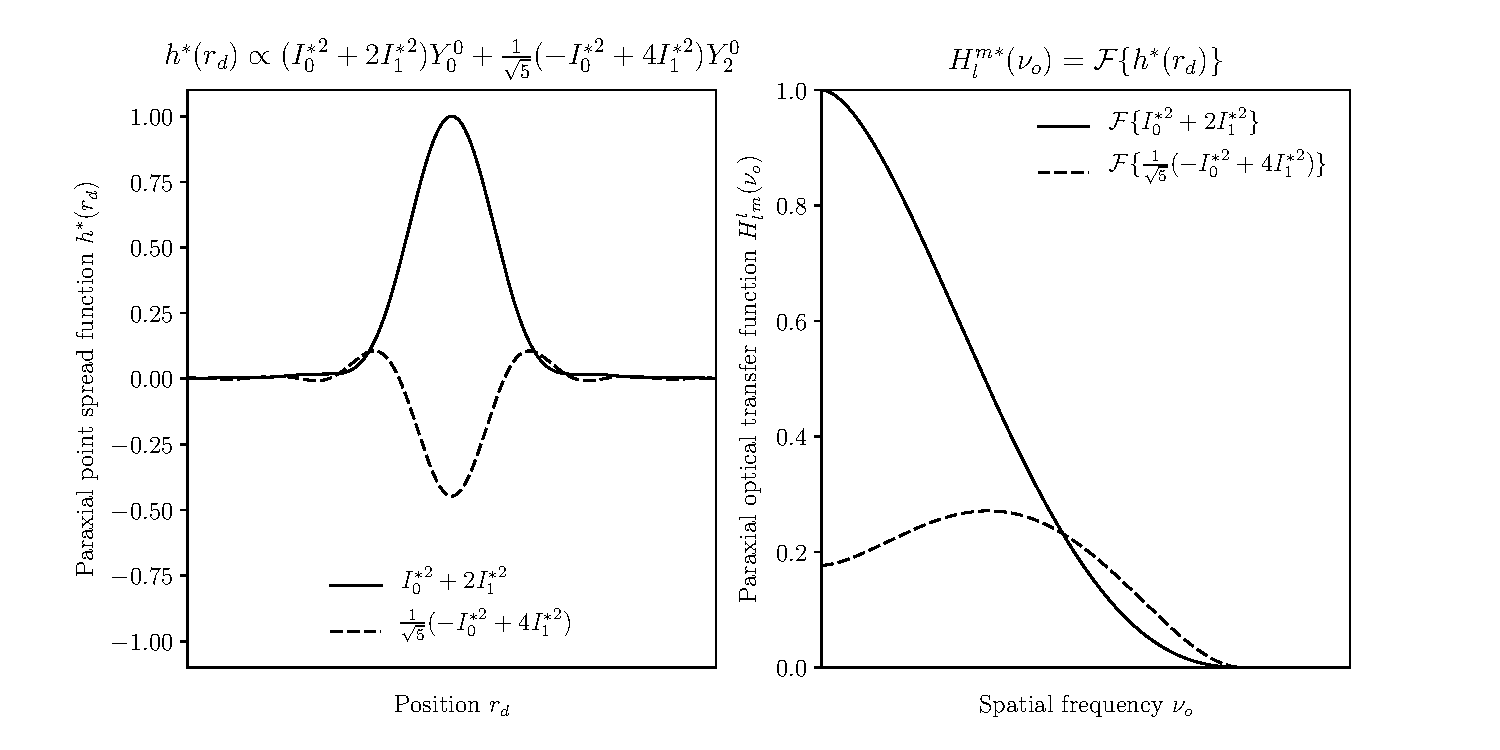
\includegraphics[width = 1.\textwidth]{../calculations/ft.pdf}
   \caption{In progress. \textbf{Left:} Paraxial spatio-angular point spread
     function for a single-view fluorescence microscope with NA=0.8. The solid
     line is the PSF for $y_0^0$ distributions and the dashed line is the PSF
     for $y_2^0$ distributions. $y_2^0$ includes ``negative'' fluorophores, so
     it gives rise to a negative PSF. \textbf{Right:} Numerical paraxial
     spatio-angular optical transfer function for the same microscope. The
     $y_0^0$ term has a spatial low-pass response while the $y_2^0$ term has a
     spatial high-pass response. The relative sizes of the two terms is set by
     the NA---increasing the NA increases the relative size of the $y_0^2$ term.
     Vertical scaling is correct---horizontal scaling is in progress. The cutoff
     frequency is proportional to NA and is the same for both spherical harmonic
     terms.}
   \label{fig:para}
\end{figure}
    
\section{Conclusions}

TODO 

\bibliography{report}{}
\bibliographystyle{unsrt}

\appendix
\section{Products of real spherical harmonics}\label{realspherical}
The six products of $l=1$ spherical harmonics are
\begin{align}
y_1^{-1}y_1^{-1}\sqrt{\pi} &= \frac{1}{2 }y_0^0 + - \frac{\sqrt{5}}{10 }y_2^0 + - \frac{\sqrt{15}}{10 }y_2^2,\\ 
y_1^{-1}y_1^0\sqrt{\pi} &= \frac{\sqrt{15}}{10 }y_2^{-1} ,\\
y_1^{-1}y_1^1\sqrt{\pi} &= - \frac{\sqrt{15}}{10 }y_2^{-2} ,\\
y_1^0y_1^0\sqrt{\pi} &= \frac{1}{2 }y_0^0 + \frac{\sqrt{5}}{5 }y_2^0 ,\\
y_1^0y_1^1\sqrt{\pi} &= \frac{\sqrt{15}}{10 }y_2^1 ,\\
y_1^1y_1^1\sqrt{\pi} &= \frac{1}{2 }y_0^0 + - \frac{\sqrt{5}}{10 }y_2^0 + \frac{\sqrt{15}}{10 }y_2^2.
\end{align}
The fifteen products of $l=2$ spherical harmonics are
\begin{align}
y_2^{-2}y_2^{-2}\sqrt{\pi} &= \frac{1}{2 }y_0^{0} + - \frac{\sqrt{5}}{7 }y_2^{0} + \frac{1}{14 }y_4^{0} + - \frac{\sqrt{35}}{14 }y_4^{4} \\
y_2^{-2}y_2^{-1}\sqrt{\pi} &= - \frac{\sqrt{15}}{14 }y_2^{1} + \frac{\sqrt{10}}{28 }y_4^{1} + \frac{\sqrt{70}}{28 }y_4^{3} \\
y_2^{-2}y_2^{0}\sqrt{\pi} &= - \frac{\sqrt{5}}{7 }y_2^{-2} + \frac{\sqrt{15}}{14 }y_4^{-2} \\
y_2^{-2}y_2^{1}\sqrt{\pi} &= - \frac{\sqrt{15}}{14 }y_2^{-1} + - \frac{\sqrt{70}}{28 }y_4^{-3} + \frac{\sqrt{10}}{28 }y_4^{-1} \\
y_2^{-2}y_2^{2}\sqrt{\pi} &= \frac{\sqrt{35}}{14 }y_4^{-4} \\
y_2^{-1}y_2^{-1}\sqrt{\pi} &= \frac{1}{2 }y_0^{0} + \frac{\sqrt{5}}{14 }y_2^{0} + - \frac{\sqrt{15}}{14 }y_2^{2} + - \frac{2}{7 }y_4^{0} + - \frac{\sqrt{5}}{7 }y_4^{2} \\
y_2^{-1}y_2^{0}\sqrt{\pi} &= \frac{\sqrt{5}}{14 }y_2^{-1} + \frac{\sqrt{30}}{14 }y_4^{-1} \\
y_2^{-1}y_2^{1}\sqrt{\pi} &= - \frac{\sqrt{15}}{14 }y_2^{-2} + - \frac{\sqrt{5}}{7 }y_4^{-2} \\
y_2^{-1}y_2^{2}\sqrt{\pi} &= - \frac{\sqrt{15}}{14 }y_2^{-1} + \frac{\sqrt{70}}{28 }y_4^{-3} + \frac{\sqrt{10}}{28 }y_4^{-1} \\
y_2^{0}y_2^{0}\sqrt{\pi} &= \frac{1}{2 }y_0^{0} + \frac{\sqrt{5}}{7 }y_2^{0} + \frac{3}{7 }y_4^{0} \\
y_2^{0}y_2^{1}\sqrt{\pi} &= \frac{\sqrt{5}}{14 }y_2^{1} + \frac{\sqrt{30}}{14 }y_4^{1} \\
y_2^{0}y_2^{2}\sqrt{\pi} &= - \frac{\sqrt{5}}{7 }y_2^{2} + \frac{\sqrt{15}}{14 }y_4^{2} \\
y_2^{1}y_2^{1}\sqrt{\pi} &= \frac{1}{2 }y_0^{0} + \frac{\sqrt{5}}{14 }y_2^{0} + \frac{\sqrt{15}}{14 }y_2^{2} + - \frac{2}{7 }y_4^{0} + \frac{\sqrt{5}}{7 }y_4^{2} \\
y_2^{1}y_2^{2}\sqrt{\pi} &= \frac{\sqrt{15}}{14 }y_2^{1} + - \frac{\sqrt{10}}{28 }y_4^{1} + \frac{\sqrt{70}}{28 }y_4^{3} \\
y_2^{2}y_2^{2}\sqrt{\pi} &= \frac{1}{2 }y_0^{0} + - \frac{\sqrt{5}}{7 }y_2^{0} + \frac{1}{14 }y_4^{0} + \frac{\sqrt{35}}{14 }y_4^{4}
\end{align}
  
\section{Paraxial optical transfer function in terms of elementary functions}\label{paraxialotf}
In progress. 

Our goal is to calculate the paraxial optical transfer function. We start by
plugging Eq. \ref{eq:kernel} into Eq. \ref{eq:ft}, using the paraxial
approximation, and constraining ourselves to the transverse plane
\begin{align}
  {H_l^m}^{(p)}(\bs{\nu}_o) = \int_{\mathbb{R}^2}d\mb{r}_o{} \int_{\mathbb{S}^2}d\so{}\ \left|\int_{\mathbb{R}^2} d\rb{}\, \mb{e}_b(\rb{}; \ro{}, \so{})\me^{-i (kn_t/f_t) \rb{} \cdot \rd{}}\right|^2
 y_l^m(\so{})\thinspace\me^{i 2\pi \ro{}\cdot\bs{\nu}_o}\label{eq:ft2}.
\end{align}
We change the order of the integrals
\begin{align}
  {H_l^m}^{(p)}(\bs{\nu}_o) = \int_{\mathbb{S}^2}d\so{}\ y_l^m(\so{}) \int_{\mathbb{R}^2}d\mb{r}_o\ \left|\int_{\mathbb{R}^2} d\rb{}\, \mb{e}_b(\rb{}; \ro{}, \so{})\me^{-i (kn_t/f_t) \rb{} \cdot \rd{}}\right|^2 \me^{i 2\pi \ro{}\cdot\bs{\nu}_o}, 
\end{align}
then apply the Wiener-Khinchin theorem
$\mathcal{F}\{|\mathcal{F}\{\mb{e}_b\}|^2\} = \mb{e}_b \star \mb{e}_b$ to find
that
\begin{align}
  H_l^m(\bs{\nu}_o) = \int_{\mathbb{S}^2}d\so{}\ y_l^m(\so{}) \left[\mb{e}_b \star \mb{e}_b\right](\bs{\nu}_o). 
\end{align}
The vector auto-correlation is given by
\begin{align}
[\mb{e}_b \star \mb{e}_b](\bs{\nu}_o) = \int_{\mathbb{R}^2}d\bs{r}_b \mb{e}_b^{T}(\bs{r}_b)\mb{e}_b(\bs{r}_b + \bs{\nu}_o),
\end{align}
where $\cdot^T$ denotes the transpose operator. 

\end{document}

